\documentclass[main.tex]{subfiles}

\begin{document}
\subsection{PID Implementation}
The open-loop stability analysis indicated that the linearized system contains an unstable pole associated with the mechanical dynamics of the inverted pendulum. In addition, the control voltage affects the pendulum angle only indirectly through the coil current, which introduces internal electrical dynamics. As a result, the system indicates a weak coupling between the control input and the mechanical output.

This structure has important implications for controller design. In particular, it suggests that directly applying a single-loop PID controller from the pendulum angle to the actuator voltage may lead to poor closed-loop performance or instability. To investigate this limitation, a classical single-loop PID controller is first implemented and evaluated.

\subsubsection{Single-loop PID Control}
In the single-loop PID configuration, the pendulum angle is used as the feedback signal. Based on that feedback, the controller directly supplies the actuator voltage. The controller structure follows the classic PID design described in the previous section.

The controller is applied to the linearized continuous-time model of the system, and the closed-loop response is evaluated through time-domain simulations.

\begin{figure}[hbt!]
    \centering
    \includegraphics[width=0.75\linewidth]{single_loop PID.png}
    \caption{Single-loop PID control}
    \label{fig:singlePID}
\end{figure}

The simulation results in \cref{fig:singlePID} show that the single-loop PID controller does not stabilize the system robustly. Depending on the chosen gains, the response either diverges or exhibits excessively large oscillations and control effort. This behavior is caused by the system architecture itself rather than poor tuning. The electromagnetic actuator introduces an additional integrator between the control input and mechanical states. That significantly limits the effectiveness of a single-loop PID design. 

Based on these observations, the single-loop PID controller is unsuitable for the considered system.

\subsubsection{Cascaded PID Control}

The analysis of the single-loop PID control in previous section indicates that this design does not suit the purpose of pendulum stabilization. That motivates the consideration of a cascaded PID architecture. This design splits the system into two subsystems: an inner electrical loop and an outer mechanical loop. This aligns with the physical structure of the system and allows each subsystem to be controlled independently.

In cascaded PID architecture in \cref{fig:cascadedblock}, the inner loop controls the coil current using a PI controller what ensures stable electrical dynamics. The outer loop controls the pendulum angle using a PD controller and sets the current reference for the inner loop \cite{caspid}. Such a separation of the system effectively improves the coupling between the control input and the mechanical states and addresses the instability identified in the open-loop analysis. 

\begin{figure}[hbt!]
\centering
\resizebox{\linewidth}{!}{
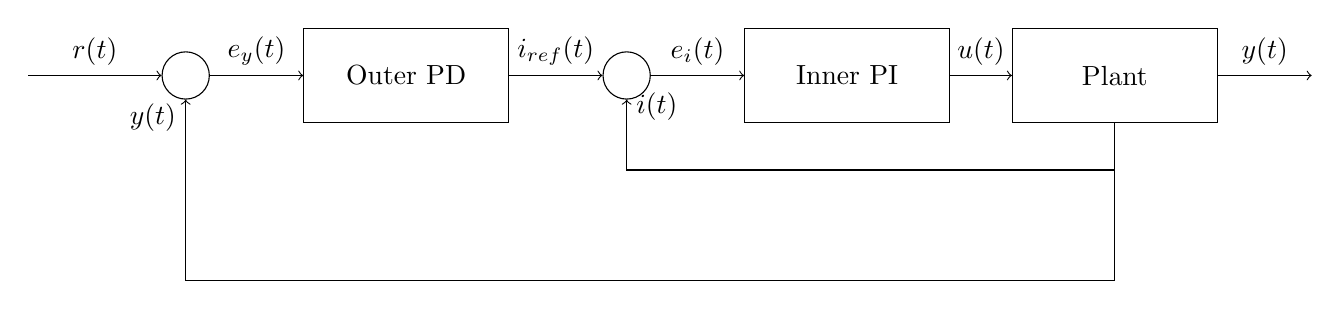
\begin{tikzpicture}[auto, node distance=2cm]

% Styles
\tikzstyle{block} = [draw, rectangle, minimum height=1.2cm, minimum width=2.6cm]
\tikzstyle{sum}   = [draw, circle, inner sep=0pt, minimum size=6mm]
\tikzstyle{input} = [coordinate]
\tikzstyle{output}= [coordinate]

% Nodes
\node [input, name=r] {};
\node [sum, right of=r] (sum1) {};
\node [block, right of=sum1, node distance=2.8cm] (pd) {Outer PD};
\node [sum, right of=pd, node distance=2.8cm] (sum2) {};
\node [block, right of=sum2, node distance=2.8cm] (pi) {Inner PI};
\node [block, right of=pi, node distance=3.4cm] (plant) {Plant};
\node [output, right of=plant, node distance=2.5cm] (y) {};

% Feedback coordinates (IMPORTANT)
\node [coordinate, below of=plant, node distance=1.2cm] (fb_i) {};
\node [coordinate, below of=plant, node distance=2.6cm] (fb_y) {};

% Forward path
\draw [->] (r) -- node {$r(t)$} (sum1);
\draw [->] (sum1) -- node {$e_y(t)$} (pd);
\draw [->] (pd) -- node {$i_{\text{ref}}(t)$} (sum2);
\draw [->] (sum2) -- node {$e_i(t)$} (pi);
\draw [->] (pi) -- node {$u(t)$} (plant);
\draw [->] (plant) -- node {$y(t)$} (y);

% Inner loop (current)
\draw [->] (plant) -- (fb_i) -| node[pos=0.95, right] {$i(t)$} (sum2);

% Outer loop (output)
\draw [->] (plant) -- (fb_y) -| node[pos=0.95, left] {$y(t)$} (sum1);

\end{tikzpicture}
}
\caption{Cascaded PID control block diagram}
\label{fig:cascadedblock}
\end{figure}

\subsubsection{MATLAB implementation}
The term appearing in the linearized state matrix that couples the coil current to the angular acceleration is
\begin{equation}
    \frac{2ki_0}{mld^2}.
\end{equation}

This term represents the linearized effect of the electromagnetic actuation on the pendulum dynamics. For convenience, this coupling term is denoted by the parameter $\alpha$ in the subsequent controller implementation, such that

\begin{equation}
    \alpha = \frac{2ki_0}{mld^2}.
\end{equation}

The value of $\alpha$ depends on the system parameters and the chosen equilibrium point. For the parameter values considered in this project, $\alpha$ evaluates to approximately 2 and is therefore used as a constant parameter in the controller simulation. This simplification allows the focus to remain on the control design and performance comparison rather than on detailed parameter identification.

The cascaded PID controller is simulated by numerically integrating the closed-loop system dynamics using ode45. This MATLAB function solves the continuous-time state-space equations and provides the time-domain response of the system.

The extract of the script with the main logic:
\begin{lstlisting}[
frame=single,
numbers=left,
style=Matlab-Pyglike]
% Params
g  = 9.81;
l  = 0.2;
R  = 4.0;
Lc = 0.02;

alpha = 2.0;

%% Controller gains
Kp_phi = 40;
Kd_phi = 8;

Kp_i = 20;
Ki_i = 400;

% Initial conditions
phi0     = 0.05;
phiDot0 = 0.0;
i0       = 0.0;
z_i0     = 0.0;

x0 = [phi0; phiDot0; i0; z_i0];

% Simulation
tspan = [0 5];

[t, x] = ode45(@(t,x) cascadedPID_ode(t,x,...
    g,l,R,Lc,alpha,...
    Kp_phi,Kd_phi,...
    Kp_i,Ki_i), tspan, x0);

\end{lstlisting}


\subsubsection{Closed-loop Performance of Cascaded PID}

The cascaded PID controller is implemented using the linearized continuous-time model. Time-domain simulations demonstrate that the cascaded structure successfully stabilizes the inverted pendulum around the upright equilibrium.

\begin{figure}[hbt!]
    \centering
    \includegraphics[width=0.75\linewidth]{cascaded_PID.png}
    \caption{Closed-loop Cascaded PID}
    \label{fig:cascadedPID}
\end{figure}

Compared to the single-loop PID, the cascaded controller in \cref{fig:cascadedPID} exhibits a well-damped response, reduced settling time, and bounded control effort. The pendulum angle converges smoothly to zero, and the current remains within acceptable limits throughout the transient.

To quantify the closed-loop behavior, standard performance metrics in \cref{fig:metrics} are evaluated, including settling time, overshoot, peak current, and RMS current.

\begin{figure}[hbt!]
    \centering
    \includegraphics[width=0.75\linewidth]{PID_metrics.png}
    \caption{Cascaded PID performance metrics}
    \label{fig:metrics}
\end{figure}

These results confirm that the cascaded PID architecture provides a significant improvement in stability and performance over the single-loop PID controller.

\subsubsection{PID tuning}

The PID gains were selected using an iterative simulation-based tuning procedure. For the single-loop PID controller, various combinations of proportional, integral, and derivative gains were tested. However, there was no set of gains able to provide robust stabilization due to the indirect coupling between the control input and the mechanical dynamics.

The cascaded PID controller was tuned sequentially. Initially, the inner current loop was tuned using a PI controller to achieve fast and stable electrical dynamics. Subsequently, the outer angle loop was tuned using a PD controller to ensure a well-damped mechanical response while keeping the required control effort within acceptable limits. Since the control architecture is cascaded, automatic tuning tools such as the MATLAB PID Tuner were not used. The PID tuner is designed for a single-loop controller configuration. The final gains were therefore selected to balance stability, transient performance, and actuator effort.

\subsubsection{Implications for the Project}

The investigation of PID-based control strategies shows that a classical single-loop PID controller is not suitable for stabilizing the electromagnetically actuated inverted pendulum due to the indirect coupling between the control input and the mechanical states. By contrast, the cascaded PID controller, motivated by the system stability analysis, effectively stabilizes the system and achieves satisfactory performance. However, the tuning of cascaded PID gains remains complex and system-specific. That motivates the exploration of a more systematic LQR controller in the next section.

\end{document}